\section{Technologie CMOS : Complementary Metal Oxyde Semiconductor}

\begin{frame}{CMOS --- Transistors CMOS }
  \begin{columns}
    \begin{column}{0.5\textwidth}  % Colonne de droite (50% de la largeur)
      \begin{alertblock}{Paradigme dominant}
        Fondement de la microélectronique numérique actuelle
      \end{alertblock}
      \begin{itemize}
        \item Association de transistors \textbf{NMOS} et \textbf{PMOS} sur un même substrat.
        \item NMOS : conduit lorsque la grille est à $V_{DD}$
        \item PMOS : conduit lorsque la grille est à $0\,$V
        \begin{itemize}
          \item Se substitue à la résistance de pull-up du NMOS.
          \item Montage \textbf{dual} : série $\rightleftarrows$ parallèle.
        \end{itemize}
        \item Effet de champ : la \textbf{tension} de grille contrôle le canal.
        \item Isolation par \textbf{oxyde de grille} $\Rightarrow$ haute impédance d'entrée.
      \end{itemize}
    \end{column}

    \begin{column}{0.5\textwidth}  % Colonne de droite (50% de la largeur)
        \begin{center}
          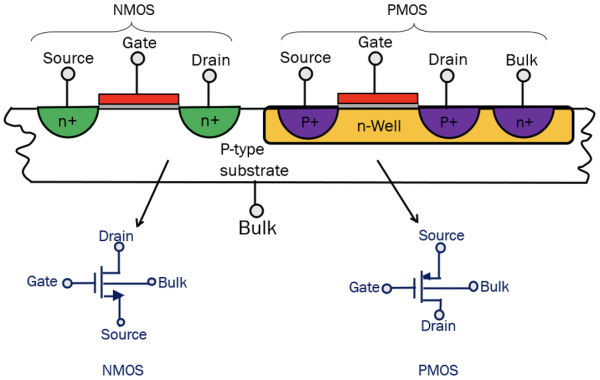
\includegraphics[scale=0.45]{./images/cmos_0.png}
        \end{center}
    \end{column}
  \end{columns}
\end{frame}

\begin{frame}{Le modèle de Schichman--Hodges : caractéristiques $I_D(V_{DS})$}

\begin{alertblock}{Physique}
 Caractérisation du comportement \textit{analogique} du MOS.
\end{alertblock}

\begin{columns}[T,totalwidth=\textwidth]

% ---------- Colonne de gauche : équations ----------
\begin{column}{0.48\textwidth}

\footnotesize
\textbf{1. Blocage} \quad ($V_{GS} - V_T \leq 0$)
\[
I_D = 0
\]

\vspace{1mm}
\textbf{2. Zone linéaire} \quad ($0 < V_{DS} < V_{GS}-V_T$)
\[
I_D = k_n \tfrac{W}{L}\!\left[(V_{GS}\!-\!V_T)V_{DS} - \tfrac{V_{DS}^2}{2}\right]\!\left(1+\lambda V_{DS}\right)
\]

\vspace{1mm}
\textbf{3. Saturation} \quad ($V_{DS} \geq V_{GS}-V_T$)
\[
I_D = \frac{k_n}{2} \frac{W}{L}(V_{GS}-V_T)^2\left(1+\lambda V_{DS}\right)
\]

\vspace{2mm}
\scriptsize
$k_n=\mu_n C_{ox}$ (transconductance) $\;\cdot\;$ $V_T$ (seuil) $\;\cdot\;$ $\lambda$ (modulation de canal) $\;\cdot\;$ $W/L$ (géométrie)

\vspace{2mm}
\footnotesize
\alert{Un seul jeu d'équations décrit tout le comportement}, du blocage à la saturation.

\end{column}

% ---------- Colonne de droite : courbes caractéristiques ----------
\begin{column}{0.52\textwidth}
  \begin{center}
    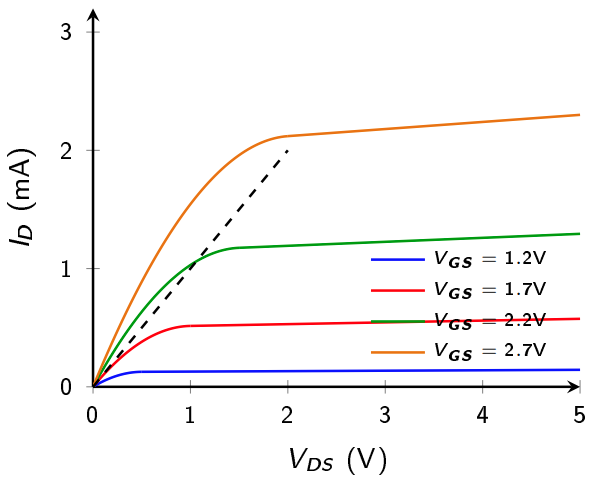
\includegraphics[scale=0.3]{./images/caract_mos.png}
  \end{center}
\end{column}

\end{columns}

\end{frame}
